\documentclass[12pt,reqno,oneside]{amsart}
% \documentclass[12pt, final]{siamonline171218}
% \usepackage[pdfborder={0 0 0.5 [3 2]}]{hyperref}%
\usepackage[left=1in,right=1in,top=1in,bottom=1.5in]{geometry}%
\usepackage{amssymb}
\usepackage{amsthm}
\usepackage{graphicx}
\usepackage{enumerate}
\usepackage{float}
\usepackage{bm}
\usepackage[stable]{footmisc}

\usepackage{packages}
\usepackage{wrapfig}
\usepackage{subfigure}
\usepackage[font=footnotesize]{caption}

\newtheorem{theorem}{Theorem}
\newtheorem{lemma}[theorem]{Lemma}
\newtheorem{corollary}{Corollary}

\theoremstyle{definition}
\newtheorem{definition}[theorem]{Definition}

\theoremstyle{remark}
\newtheorem{remark}[theorem]{Remark}

\def\noi{\noindent}
\def\T{{\mathbb T}}
\def\R{{\mathbb R}}
\def\N{{\mathbb N}}
\def\Z{{\mathbb Z}}
\def\C{{\mathbb C}}
\def\Q{\mathbb{Q}}

\DeclareMathOperator{\spn}{span}
\DeclareMathOperator{\ran}{ran}
\DeclareMathOperator{\dm}{dim}

\newcommand{\vK}{\bm{\mathit{K}}}
\newcommand{\calP}{\mathcal{P}}
\newcommand{\calA}{\mathcal{A}}

\setlength{\parindent}{0em}
\setlength{\parskip}{1em}
\renewcommand{\baselinestretch}{1.1}

\begin{document}

\thispagestyle{empty}

\section{Research Summary}

My primary research interest is solitary waves, which are localized disturbances which maintain their shape as they propagate at a constant velocity. Although they were originally discovered as a water wave phenomenon, they have applications in many fields such as fiber optics, plasma physics, and quantum mechanics; they can also be used for models in biology and neuroscience. More generally, many weakly nonlinear, dispersive PDEs have solitary wave solutions.

In particular, I study the existence and stability of multi-pulse solitary waves. These are disturbances which resemble multiple, well separated copies of a single solitary wave. In addition to having applications to fields such as nonlinear optics, multi-pulses are interesting mathematically. Since a multi-pulse structure maintains its shape as it is transmitted, it may appear at first glance that the individual pulses do not interact. The underlying dynamics, however, is inherently nonlinear, and the interaction between the pulses is revealed when we perturb the structure. I am interested in how the spectral properties of these multi-pulses can explain how they react to perturbations.

\section{Mathematical approach}

My primary mathematical approach comes from spatial dynamics. From this viewpoint, a solitary wave is a homoclinic orbit evolving in the spatial variable. This primary homoclinic orbit is an intersection of the stable and unstable manifolds of an equilibrium point, which represents the rest state of the system. Some spectral properties, such as the essential spectrum, only depend on the rest state. Multi-pulses are multi-loop homoclinic orbits, which can be constructed using Lin's method \cite{Lin2008}, a version of the Lyapunov-Schmidt method used to find solutions which remain near a homoclinic orbit. Heuristically, this process involves gluing together multiple copies of the primary homoclinic orbit. I also use Lin's method to construct periodic orbits and multi-loop periodic orbits. To find eigenvalues associated with multi-pulses, I use two main tools. First, I use Lin's method as in \cite{Sandstede1998} to construct eigenfunctions as perturbations of the eigenfunctions of the primary pulse. I also use the Krein matrix \cite{Kapitula2013a,Kap2019}, which is a projection of an eigenvalue problem onto a finite dimensional subspace.

In addition to theoretical work, I also use numerical analysis, both to generate hypotheses and to verify theoretical results. For multi-pulses, I start by constructing the primary pulse, which either involves parameter continuation from a known solution using AUTO or an energy minimization method such as the string method \cite{Chamard2011} or the mountain pass method \cite{Chen1997}. I then glue together multiple copies of the primary pulse and use a Newton solver such as Matlab's \texttt{fsolve} function to construct a multi-pulse. For the spectrum, I first discretize the problem, usually with a Fourier or polynomial spectral method. I then find the spectrum using a numerical eigenvalue solver. I also use AUTO to study how eigenvalues change as parameters are varied.

I work with the following three Hamiltonian equations in my research:
\begin{align*}
\partial_t u - \partial_x^5 u + \partial_x^3 u + 2 u \partial_x u &= 0 && \text{fifth-order Korteweg de-Vries equation (KdV5)} \\
\partial_t^2 u + \partial_x^4 u + \mathrm{e}^{u-1} - 1 &= 0 &&\text{Chen-McKenna suspension bridge equation} \\
i\partial_t u_n + d(u_{n+1} - 2 u_n + u_{n-1}) + |u_n|^2 u_n &= 0 &&\text{discrete nonlinear Schrodinger equation (dNLS)}
\end{align*}
KdV5 is a weakly nonlinear long wave approximation to capillary-gravity wave problem which also has applications to plasma physics and laser optics \cite{Pelinovsky2007}. Chen-McKenna is a smooth approximation to a model for waves propagating on an infinitely long suspended beam, and is motivated by observations of traveling waves on suspension bridges \cite{McKenna1990,Chen1997}. dNLS is the discrete analogue to the nonlinear Schrodinger equation (NLS) and has applications to nonlinear optics and condensed matter physics \cite{Kevrekidis2009}. KdV5 and Chen-McKenna have traveling wave solutions of the form $u(x, t) = \phi(x - ct)$, where $c$ is the wavespeed. dNLS has rotating waves of the form $u_n = e^{i\omega t}\phi_n$, where $\omega$ is the rotational frequency.
All three equations have primary pulse solutions \cite{Pelinovsky2007,Smets2002,Berg2018,Kevrekidis2009}. For appropriate values of the parameters $c$ and $\omega$, they also have multi-pulse solutions \cite{Buffoni1996,SandstedeStrut,Kevrekidis2009}.

\section{Interaction eigenvalues of multi-pulses}

The main focus of my research involves determining the spectrum associated with the linearization about a multi-pulse solution. In general, each pulse that is added to a multi-pulse structure is associated with one or more eigenvalues in the spectrum. I refer to these as interaction eigenvalues, since they result from nonlinear interactions between neighboring pulses. For a large class of systems, this problem is solved in \cite{Sandstede1998}, which reduces the problem of to finding the eigenvalues of a matrix.

\begin{wrapfigure}[8]{R}{6cm}
\includegraphics[width=6cm]{images/inteigpattern.eps}
\caption{Possible interaction eigenvalue patterns.} 
\label{fig:inteigpattern}
\end{wrapfigure}
The systems I study are Hamiltonian. These are not covered by the results of \cite{Sandstede1998}. The Hamiltonian structure is very helpful, since all eigenvalues must come in quartets of the form $\pm \alpha \pm \beta i$; this means that each additional set of interaction eigenvalues must come in one of the three patterns in \cref{fig:inteigpattern}. On the other hand, the presence of any eigenvalue with nonzero real part implies that there is an unstable eigenvalue. This means that Hamiltonian systems cannot be dissipative, which makes stability analysis more difficult.

My main results relate the spectral pattern of the interaction eigenvalues to the underlying geometry of the multi-pulse. For the continuous systems (KdV5 and Chen-McKenna), multi-pulses exist in discrete families. The distances between neighboring pulses are constrained to be an integer multiple of a phase parameter. This constraint is a consequence of the specific alignment of manifolds necessary for multi-pulses to occur, and these integers represent the number of twists made by the stable and unstable manifolds near the equilibrium at 0. An $m-$pulse, therefore, can be described by $m-1$ nonnegative integers $\{ k_1, \dots, k_{m-1} \}$. The eigenvalue pattern is determined by whether these integers are even or odd. For dNLS, a multi-pulse is constructed from single pulses which can either be in phase or out of phase. The eigenvalue pattern is determined by these phase differences. These patterns are illustrated in \cref{fig:eigpatterns}.

\begin{figure}
\centering
\begin{tabular}{ccc}
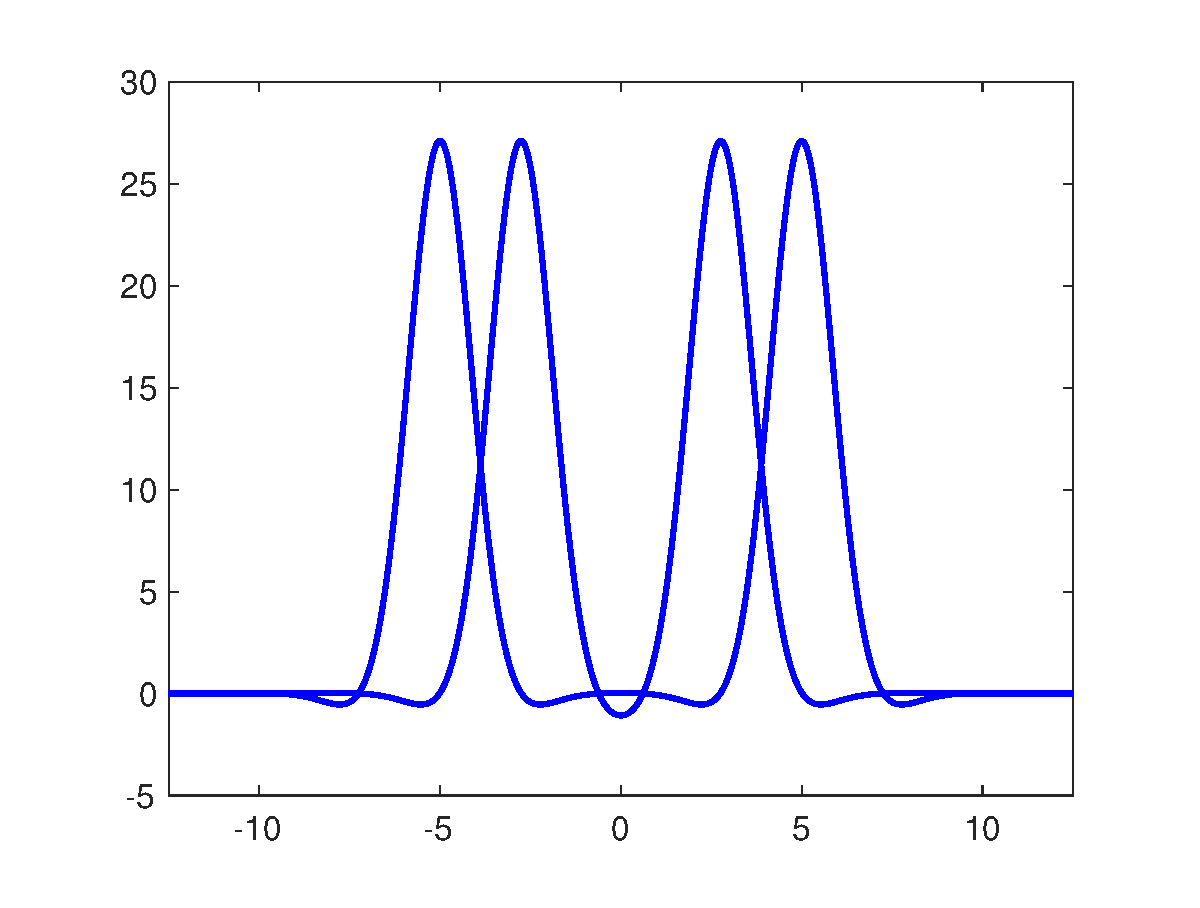
\includegraphics[width=4cm]{images/dp02.eps} &
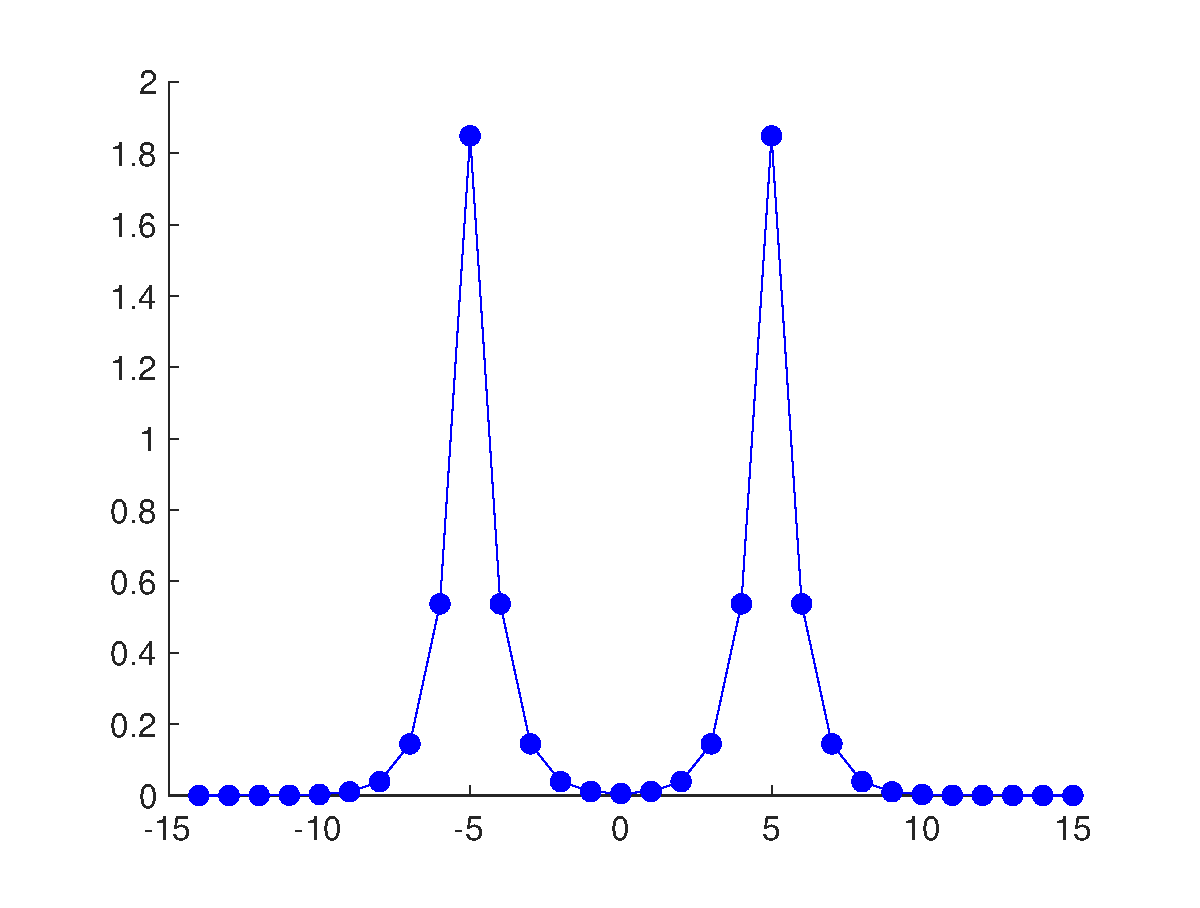
\includegraphics[width=4cm]{images/dnls2unstable.eps} &
\includegraphics[width=4cm]{images/unstableeigpattern.eps} \\
\includegraphics[width=4cm]{images/dp13.eps} &
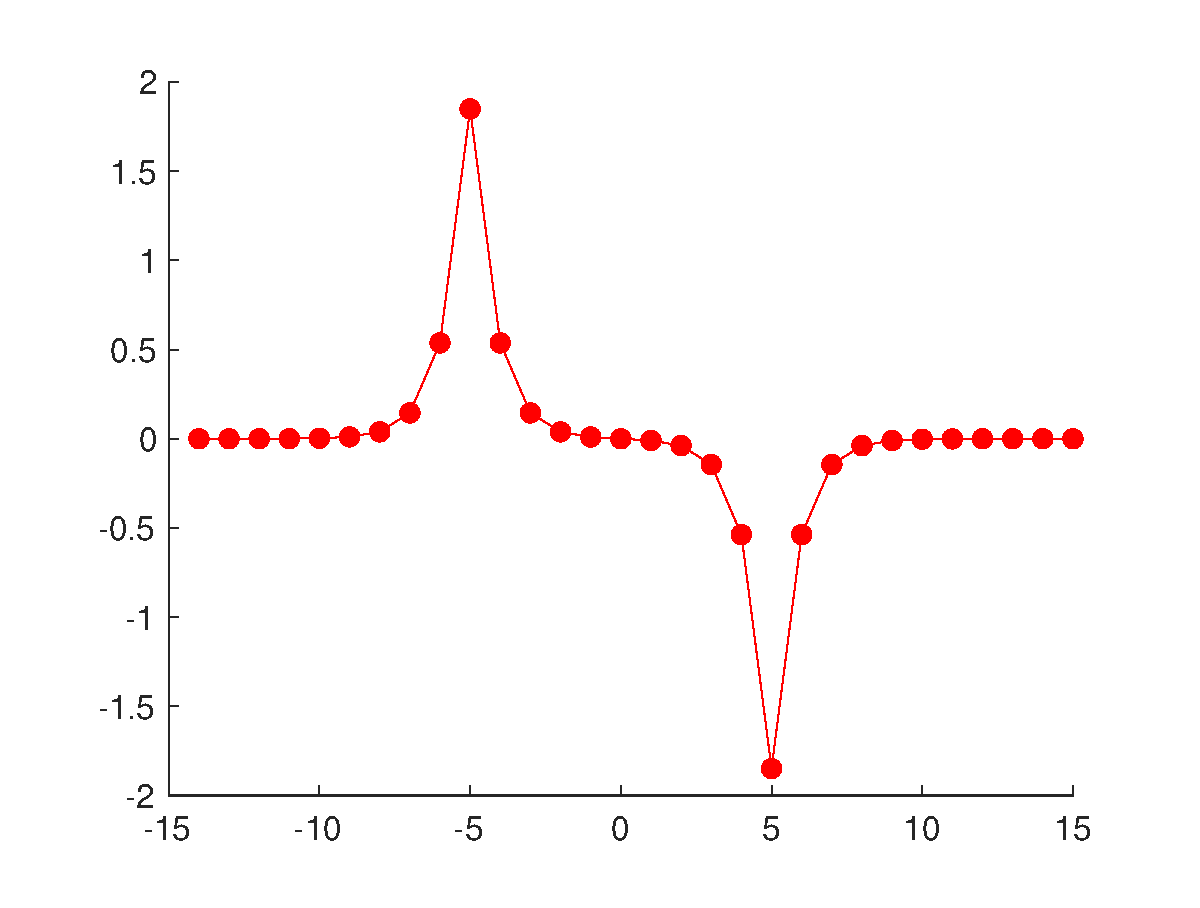
\includegraphics[width=4cm]{images/dnls2stable.eps} &
\includegraphics[width=4cm]{images/stableeigpattern.eps} 
\end{tabular}
\caption{Double pulses for KdV5 (left) and dNLS (center). Eigenvalue pattern (right).}
\label{fig:eigpatterns}
\end{figure}

I have proved these results analytically for Chen-McKenna in \cite{Kap2019} using an extension of the Krein matrix. The following theorem gives the complete spectrum for multi-pulses of Chen-McKenna. 

\begin{theorem}\label{Cheneigs}
Let $u_m(x)$ be an $m$-pulse solution to Chen-McKenna characterized by integers $\{ k_1, \dots, k_{m-1} \}$. Then as long as the pulses are sufficiently well separated:
\begin{enumerate}[(i)]
\item The essential spectrum is purely imaginary and bounded away from 0.
\item For each $k_j$ odd there is a pair of purely imaginary eigenvalues with negative Krein signature.
\item For each $k_j$ even there is a pair of real eigenvalues.
\item There is a geometrically simple eigenvalue at $\lambda = 0$ due to translation invariance.
\item All other point spectrum is purely imaginary with positive Krein signature.
\end{enumerate}
\end{theorem}

For dNLS, I use Lin's method to extend the stability results of \cite{Kapitula2001,Kapitula2001a} to solutions away from the anti-continuum limit. For KdV5, the analysis is complicated by the essential spectrum, which is the entire imaginary axis. Any purely imaginary interaction eigenvalues would be embedded in the essential spectrum. Using an exponentially weighted space, I am able to prove an instability criterion for multi-pulses. For the cases where numerical analysis suggests that there are purely imaginary interaction eigenvalues, I can only prove that they are purely imaginary to leading order. To circumvent this problem, I look at periodic multi-pulse solutions.

\section{Periodic multi-pulses}

\begin{wrapfigure}[14]{r}{0.5\textwidth}
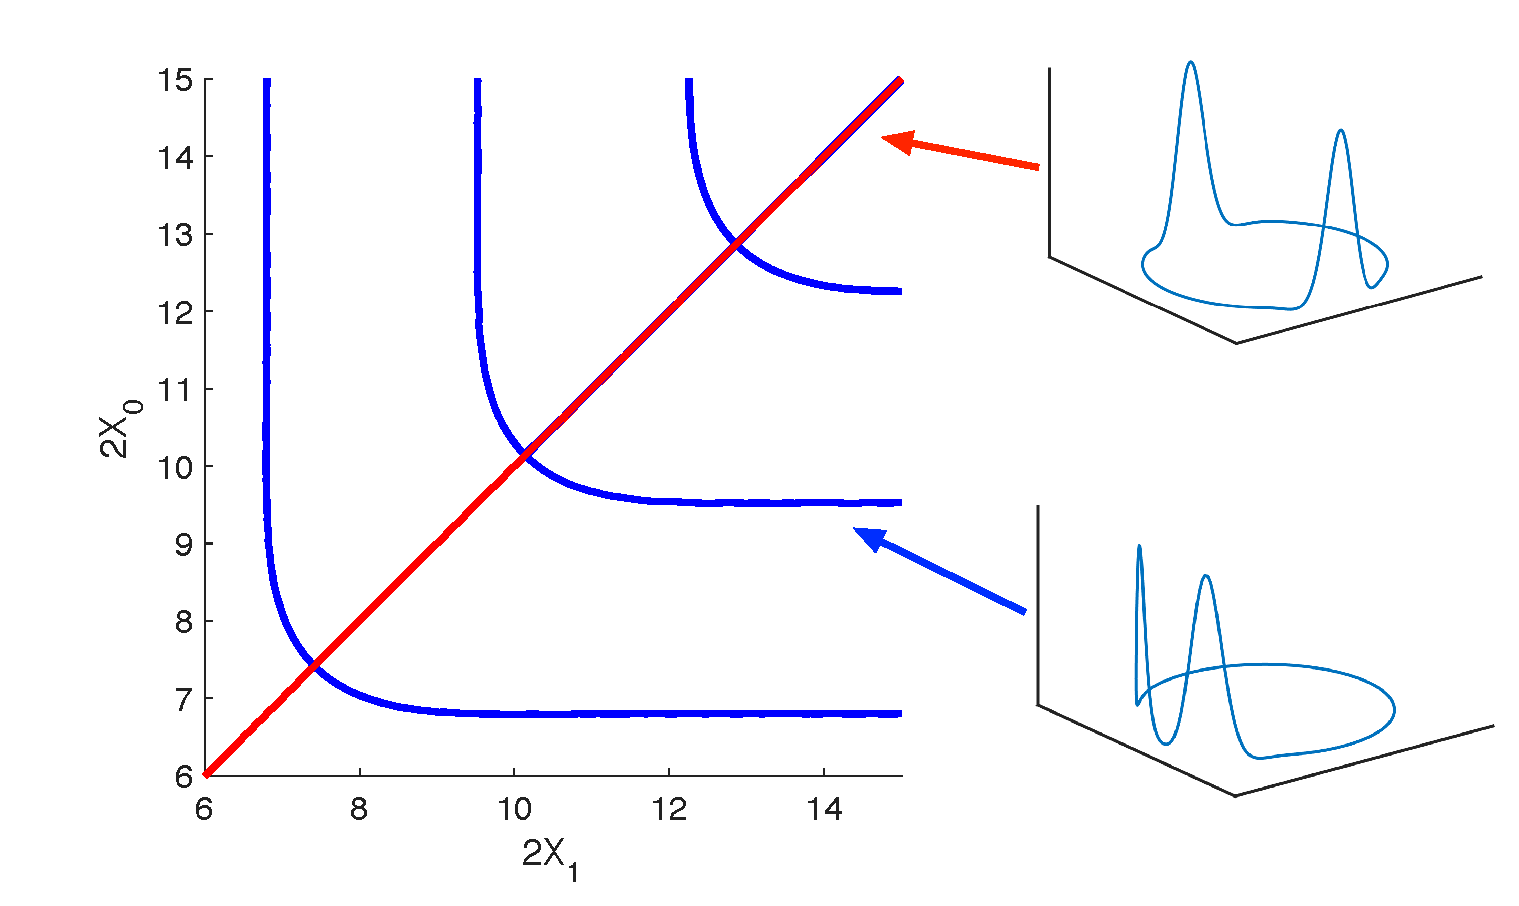
\includegraphics[width=0.5\textwidth]{images/periodicpitchforklabeled.eps}
\caption{Asymmetric periodic 2-pulses (blue) bifurcate from symmetric periodic 2-pulses (red). The distances between the two pulses are $2X_0$ and $2X_1$.
}
\label{fig:perpitchfork}
\end{wrapfigure}
A periodic multi-pulse is a periodic orbit which contains multiple peaks.  From a spatial dynamics perspective, these are multi-loop periodic orbits which are close to the primary homoclinic orbit. The advantage of looking at periodic solutions is that the essential spectrum becomes a discrete set of purely imaginary eigenvalues. These essential spectrum eigenvalues depend only on the size of the periodic domain $[-L, L]$, and we can always choose $L$ so that they stay away from the interaction eigenvalues. 

A periodic 2-pulse is constructed by gluing two single pulses together at both ends. This additional condition allows for an extra degree of freedom when compared to the ordinary 2-pulse. In particular, this means that there is a continuous family of periodic 2-pulses, as opposed to the discrete family for the ordinary 2-pulses. Asymmetric periodic 2-pulses bifurcate from symmetric periodic 2-pulses a series of pitchfork bifurcations (\cref{fig:perpitchfork}). Periodic $m-$pulses also exist for arbitrary $m$.

The eigenvalues associated with a periodic multi-pulse can be found by solving the block diagonal matrix equation
\begin{equation}\label{blockmatrix}
\det\begin{pmatrix}K(\lambda) & 0 \\ 0 & A - \lambda^2 M I \end{pmatrix} + \text{``h.o.t.''} = 0
\end{equation}
The essential spectrum eigenvalues come from the matrix $K(\lambda)$, which only depends on the background state and the domain size $L$. The interaction eigenvalues come from the matrix $A - \lambda^2 M I$, which depends on the geometry of the multi-pulse. 

\begin{wrapfigure}[15]{l}{0.5\textwidth}
\includegraphics[width=0.5\textwidth]{images/periodicequaleigbif}
\caption{Real and imaginary parts of interaction eigenvalues for symmetric periodic 2-pulses.}
\label{fig:periodicequaleigbif}
\end{wrapfigure}
For symmetric 2-pulses, there is a pair of interaction eigenvalues which is either real or purely imaginary; these collide and switch stability in a series of Hamiltonian-Hopf bifurcations which occur at the pitchfork bifurcation points (\cref{fig:periodicequaleigbif}). For asymmetric 2-periodic pulses, as long as the interaction eigenvalues and essential spectrum eigenvalues are not too close, there is a pair of interaction eigenvalues which are either real or purely imaginary. 

There is an additional complication in the periodic case. It is possible to increase $L$ so that an essential spectrum eigenvalue becomes close to an interaction eigenvalue. When this happens, I observe numerically by parameter continuation with AUTO in the domain size $L$ that there is a transient ``instability bubble'' where the two eigenvalues collide, move off of the imaginary axis temporarily, and then recombine. I call these Krein bubbles, since they result from the collision of two imaginary eigenvalues with opposite Krein signature (\cref{fig:kreinbubble1}).

\begin{wrapfigure}[13]{r}{0.45\textwidth}
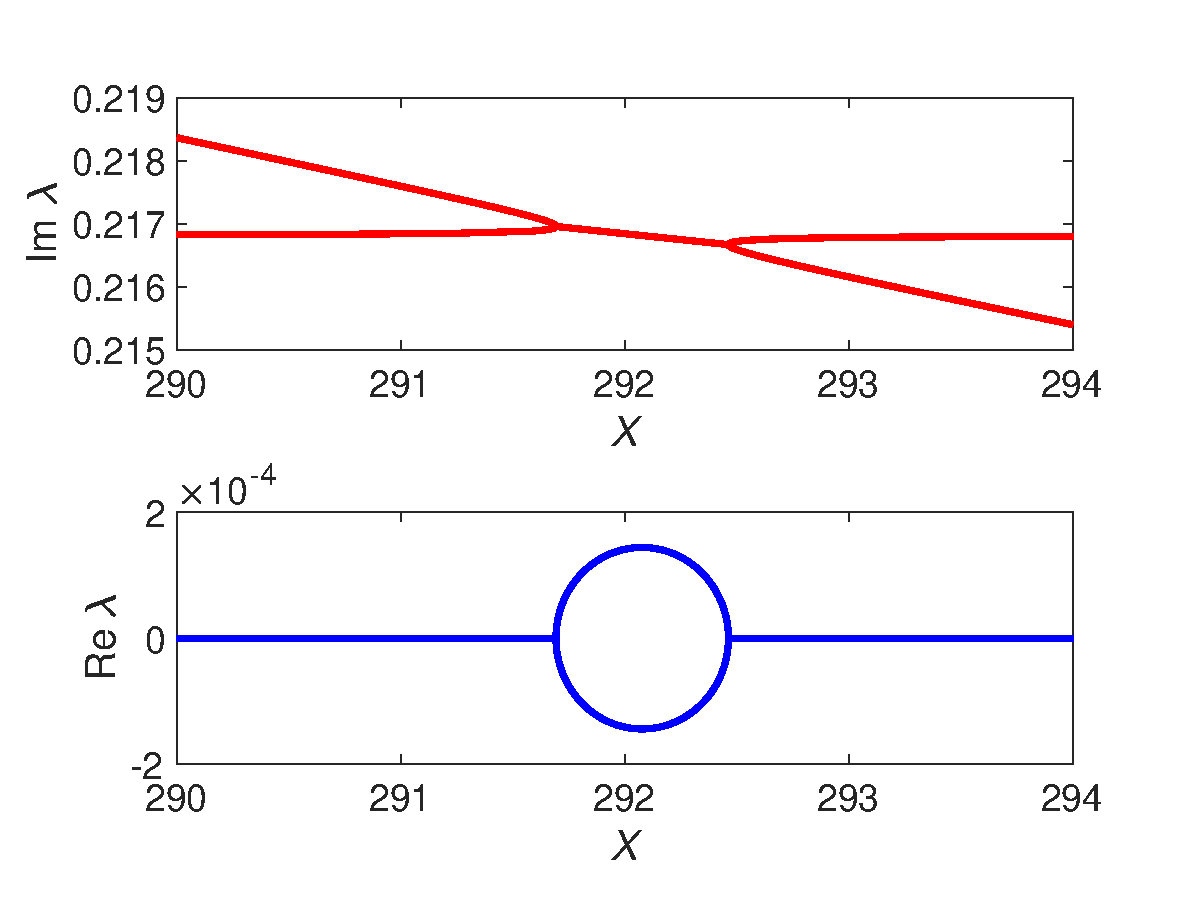
\includegraphics[width=0.45\textwidth]{images/kreinbubble1}
\caption{Collision of essential spectrum eigenvalue with purely imaginary interaction eigenvalue.}
\label{fig:kreinbubble1}
\end{wrapfigure}
Numerical analysis suggests that these Krein bubbles are small, and that their size scales as $L^{-1/2}$. I can prove that there is a radius around each purely imaginary interaction eigenvalue outside of which this cannot happen; this provides an upper bound for the size of a Krein bubble. I am currently working on proving that these instability bubbles actually exist. This involves using the symmetries of the system together with a careful analysis of the higher order terms in \eqref{blockmatrix}. Future work also includes running time-stepping simulations for 2-periodic pulses in these Krein bubbles to see what type of instability they cause.
\pagebreak
\section{Stability of multi-pulses}

How is the interaction eigenvalue pattern related to the stability of multi-pulse structures? I study this for KdV5 using numerical time-stepping, beginning with initial conditions with are close to multi-pulse solutions. At each time point, I compute the distance between the two pulses and its derivative, which I call the pulse relative velocity. I then plot trajectories of this reduced, two-dimensional system (\cref{fig:KdV5timestep}, left panel). 
\begin{figure}[H]
\begin{tabular}{cc}
\includegraphics[width=8cm]{images/phaseportrait}  &
\includegraphics[width=8cm]{images/simplephaseportrait}
\end{tabular}
\caption{Phase portrait for peak relative velocity vs. peak distance for time-stepping of KdV5 with initial conditions near the first four double pulses (left panel). Phase portrait of \cref{harmonicvary} (right panel).
}
\label{fig:KdV5timestep}
\end{figure}
For 2-pulse solutions to KdV5, there are two alternating eigenvalue patterns: unstable (pair of real interaction eigenvalues) and neutrally stable (pair of imaginary interaction eigenvalues). The unstable pattern corresponds to a saddle node; a perturbation near this equilibrium will cause the two pulses to repel each other. The stable pattern corresponds to a center; a perturbation near this equilibrium will cause the two pulses to oscillate about their center of mass. The phase portrait resembles that of the planar system \eqref{harmonicvary}, which is a harmonic oscillator with spatially varying restoring force (\cref{fig:KdV5timestep}, right panel).
\begin{equation}\label{harmonicvary}
\begin{aligned}
\dot{x} &= y \\
\dot{y} &= C e^{-\alpha_0 x} \sin \beta_0 x
\end{aligned}
\end{equation}



\bibliographystyle{amsplain}
\bibliography{researchstatement.bib}

\end{document}
